\documentclass[11pt,a4paper]{article}
\usepackage{hyperref}
\usepackage{graphicx}

\graphicspath{ {./images/} }

\begin{document}

\title{Usage of GitHub Co-pilot in our AI course project}
\author{
    Ahmed Wael \and Adham Hazem \and Omar Brikaa \and Mootaz Medhat \and Ali Esmat
}
\date{\today}
\maketitle

\section{Introduction}
Using Prolog as our programming language of choice for the AI course project,
we have found some advantages and disadvantages of using GitHub Co-pilot to auto-generate code.

\section{Advantages}
We have mostly found GitHub Co-pilot\footnote{https://github.com/features/copilot} to suggest correct code completion
in two cases:
avoiding manually typing code that does not require cognitive effort
(figures \ref{fig:copilot_html}, \ref{fig:copilot_dictionary}),
and helping in the completion of commonly typed utility code
(figures \ref{fig:copilot_subset}, \ref{fig:copilot_maximum}).

Even if the code that Co-pilot generated in these cases was not used as is, it was a good starting point.

\begin{figure}
    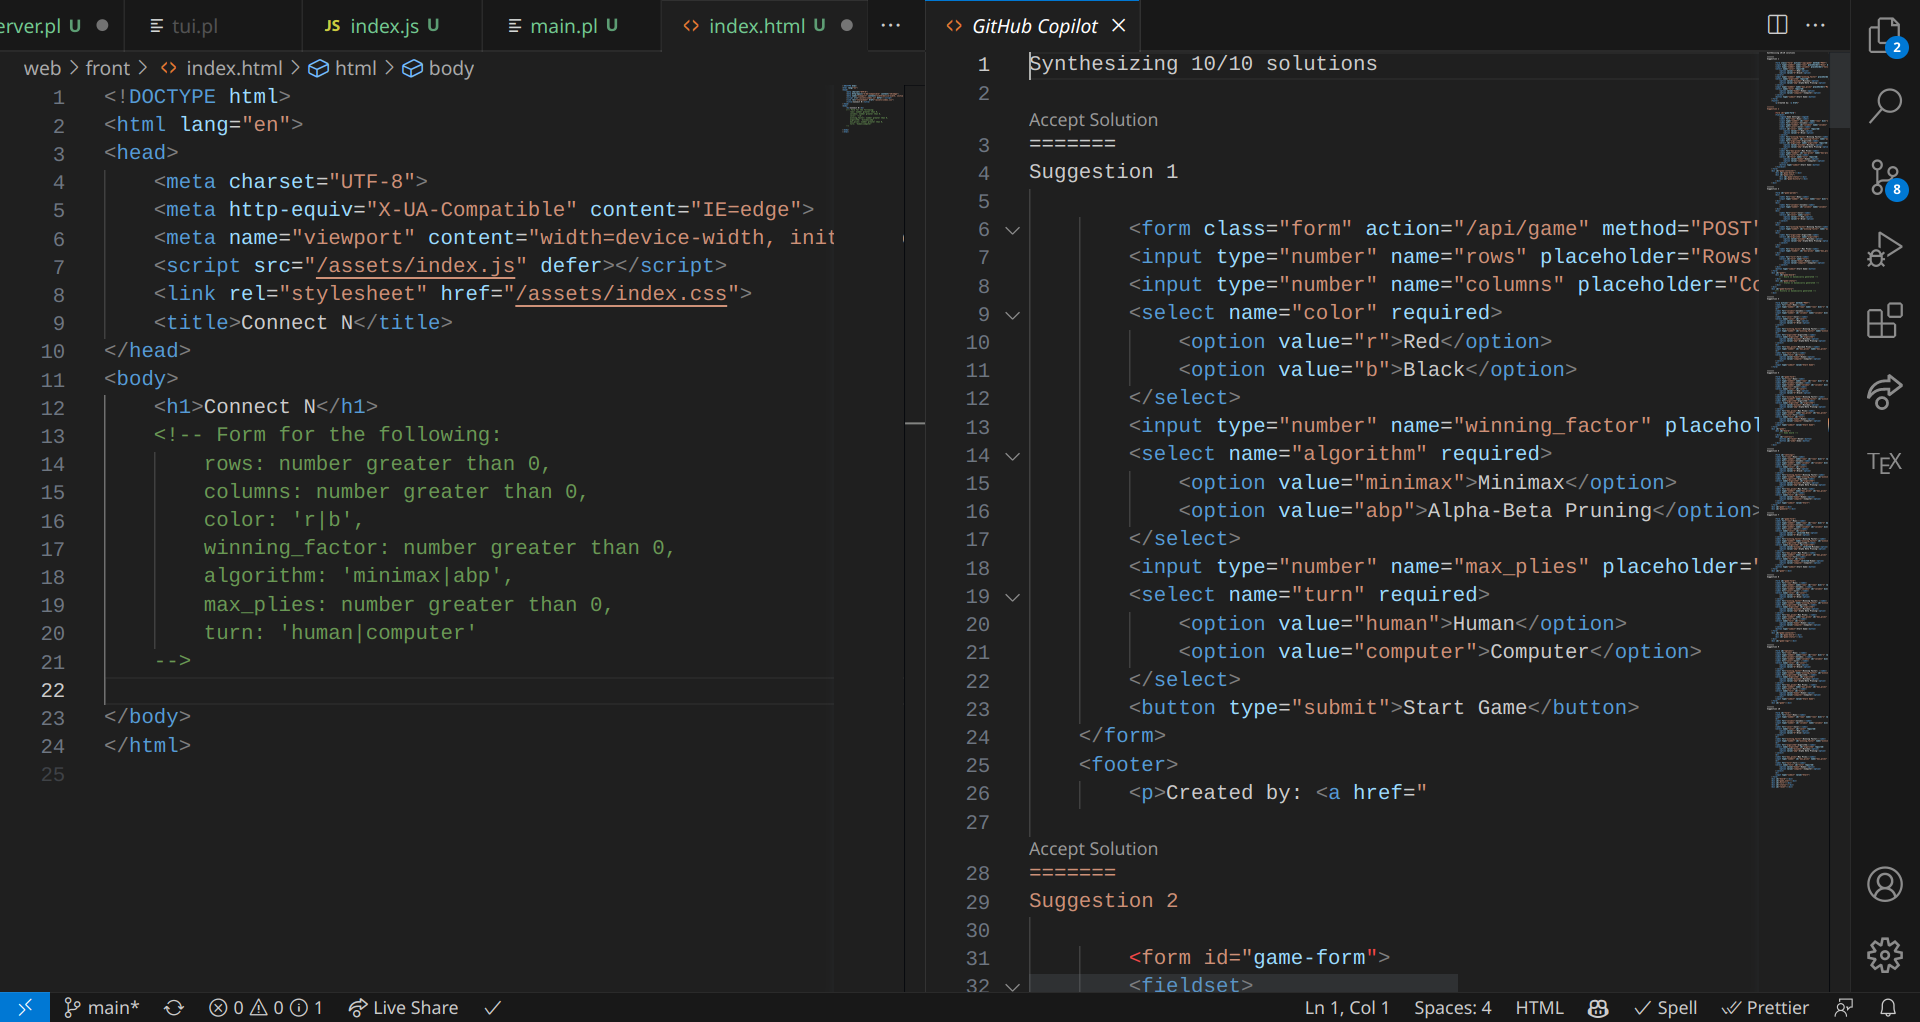
\includegraphics[width=\textwidth]{copilot-helpful-html}
    \caption{GitHub co-pilot auto-completing an HTML form based on a requirements comment (helpful)}
    \label{fig:copilot_html}
\end{figure}

\begin{figure}
    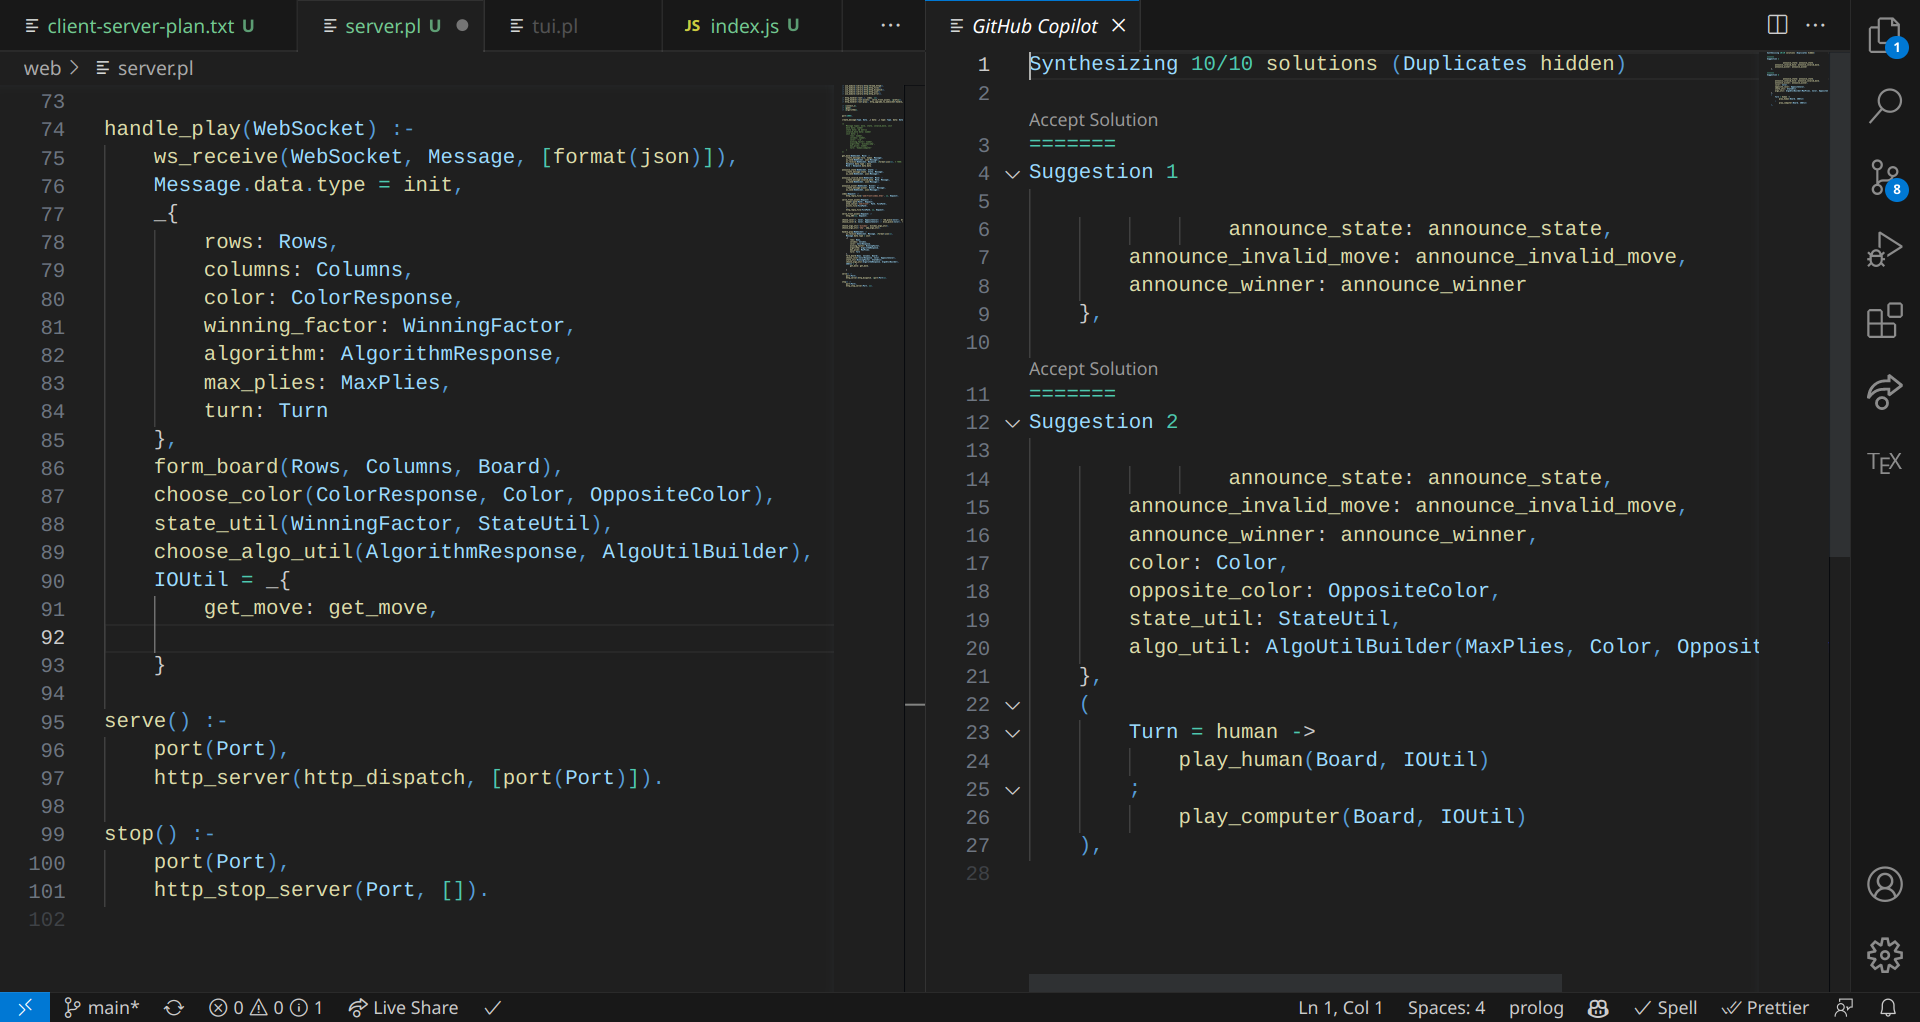
\includegraphics[width=\textwidth]{copilot-helpful-configuration-boilerplate}
    \caption{GitHub co-pilot auto-completing a configuration dictionary (helpful)}
    \label{fig:copilot_dictionary}
\end{figure}

\begin{figure}
    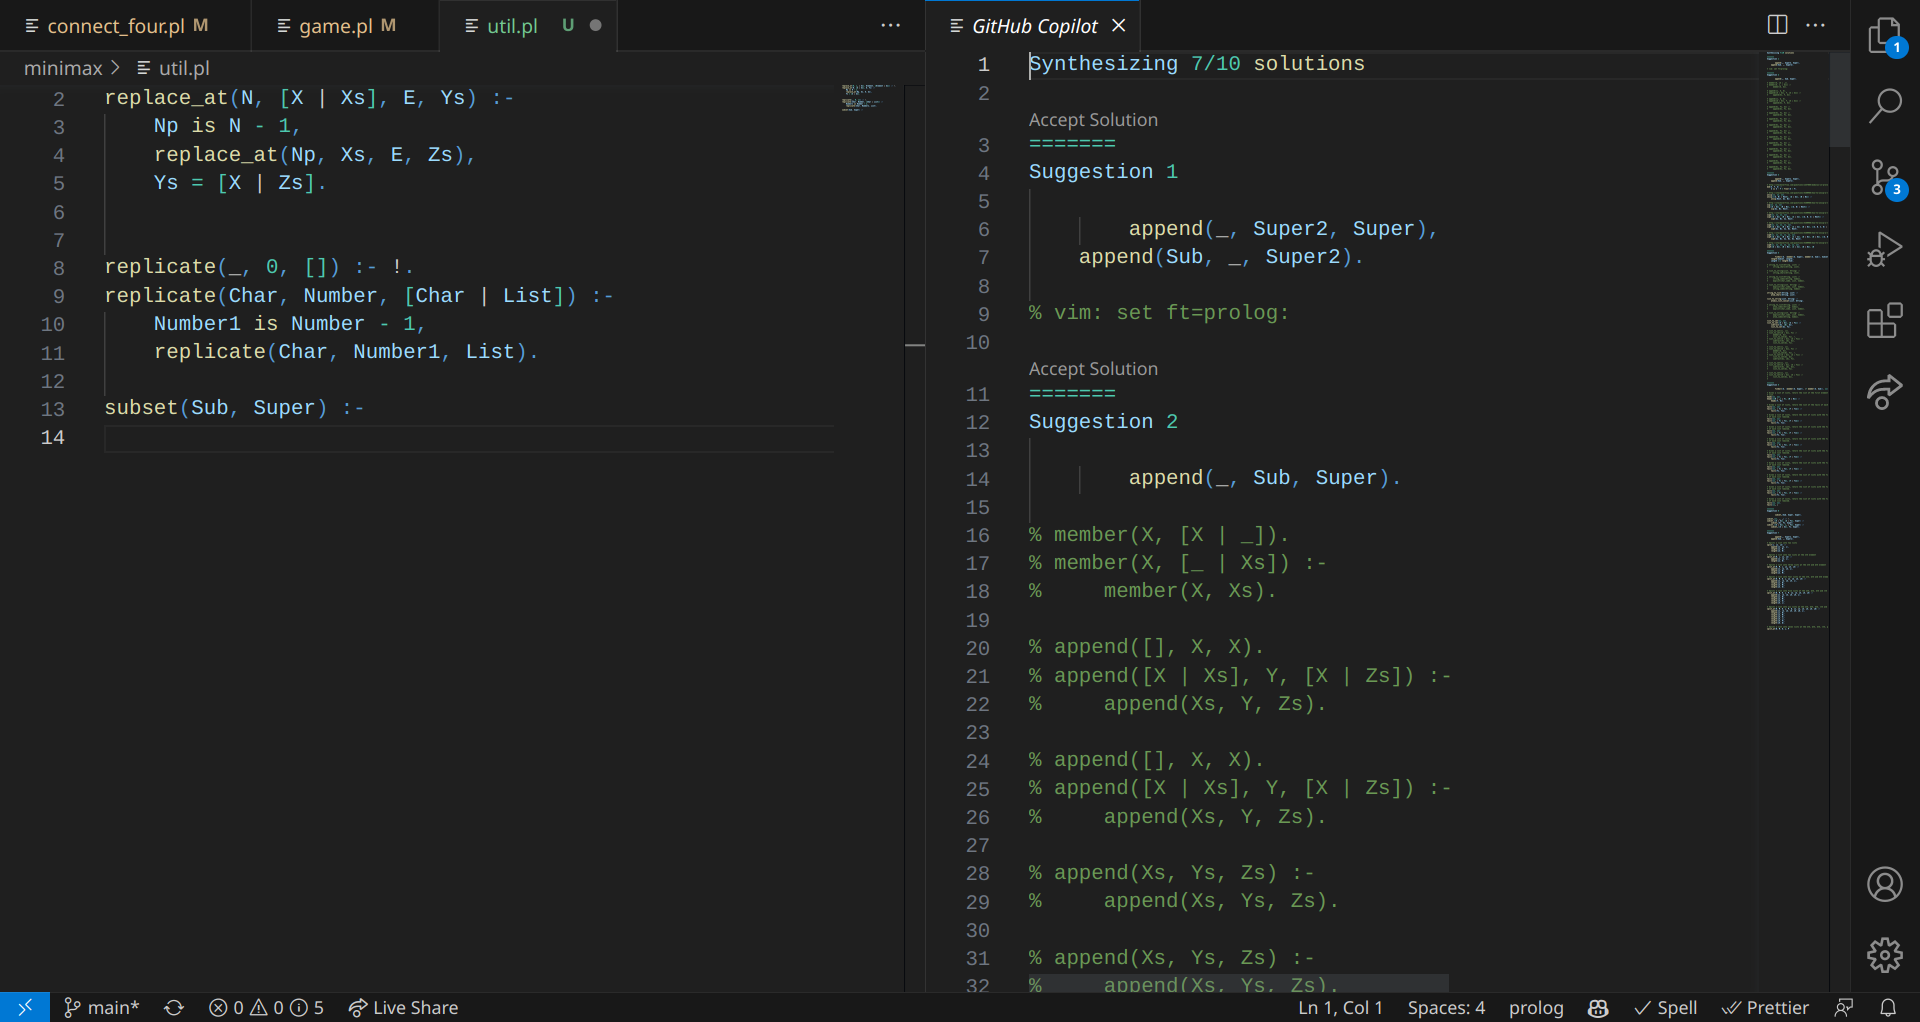
\includegraphics[width=\textwidth]{copilot-helpful-subset-predicate}
    \caption{GitHub co-pilot auto-completing the commonly used subset utility predicate (helpful)}
    \label{fig:copilot_subset}
\end{figure}

\begin{figure}
    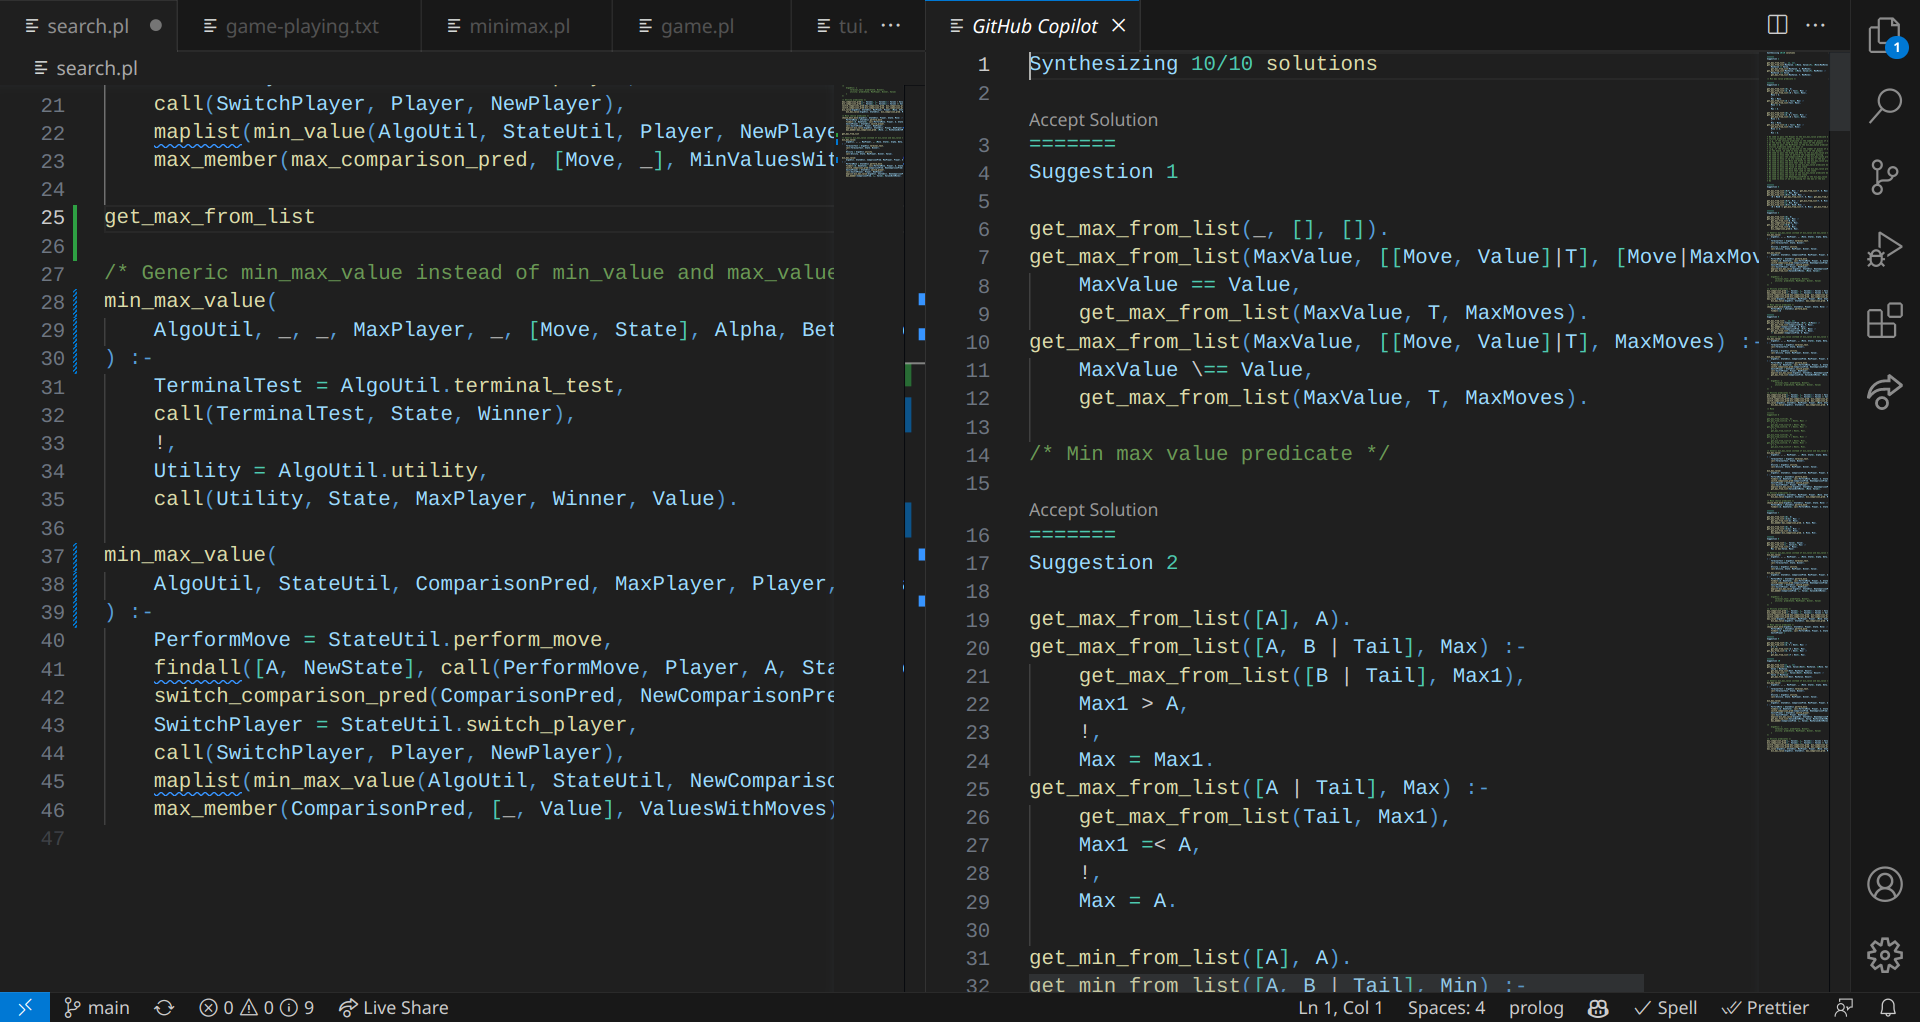
\includegraphics[width=\textwidth]{copilot-helpful-maximum-predicate}
    \caption{GitHub co-pilot auto-completing the commonly used maximum from list predicate (helpful)}
    \label{fig:copilot_maximum}
\end{figure}

\section{Disadvantages}
We have mostly found GitHub Co-pilot to generate inaccurate code in codebase-specific algorithms that aren't commonly
used in other projects (figure \ref{fig:copilot_diagonal}).

Moreover, Co-pilot does not suggest code refactoring and would suggest duplicate code if the programmer does not exert
effort to maintain the quality of their codebase.

\begin{figure}
    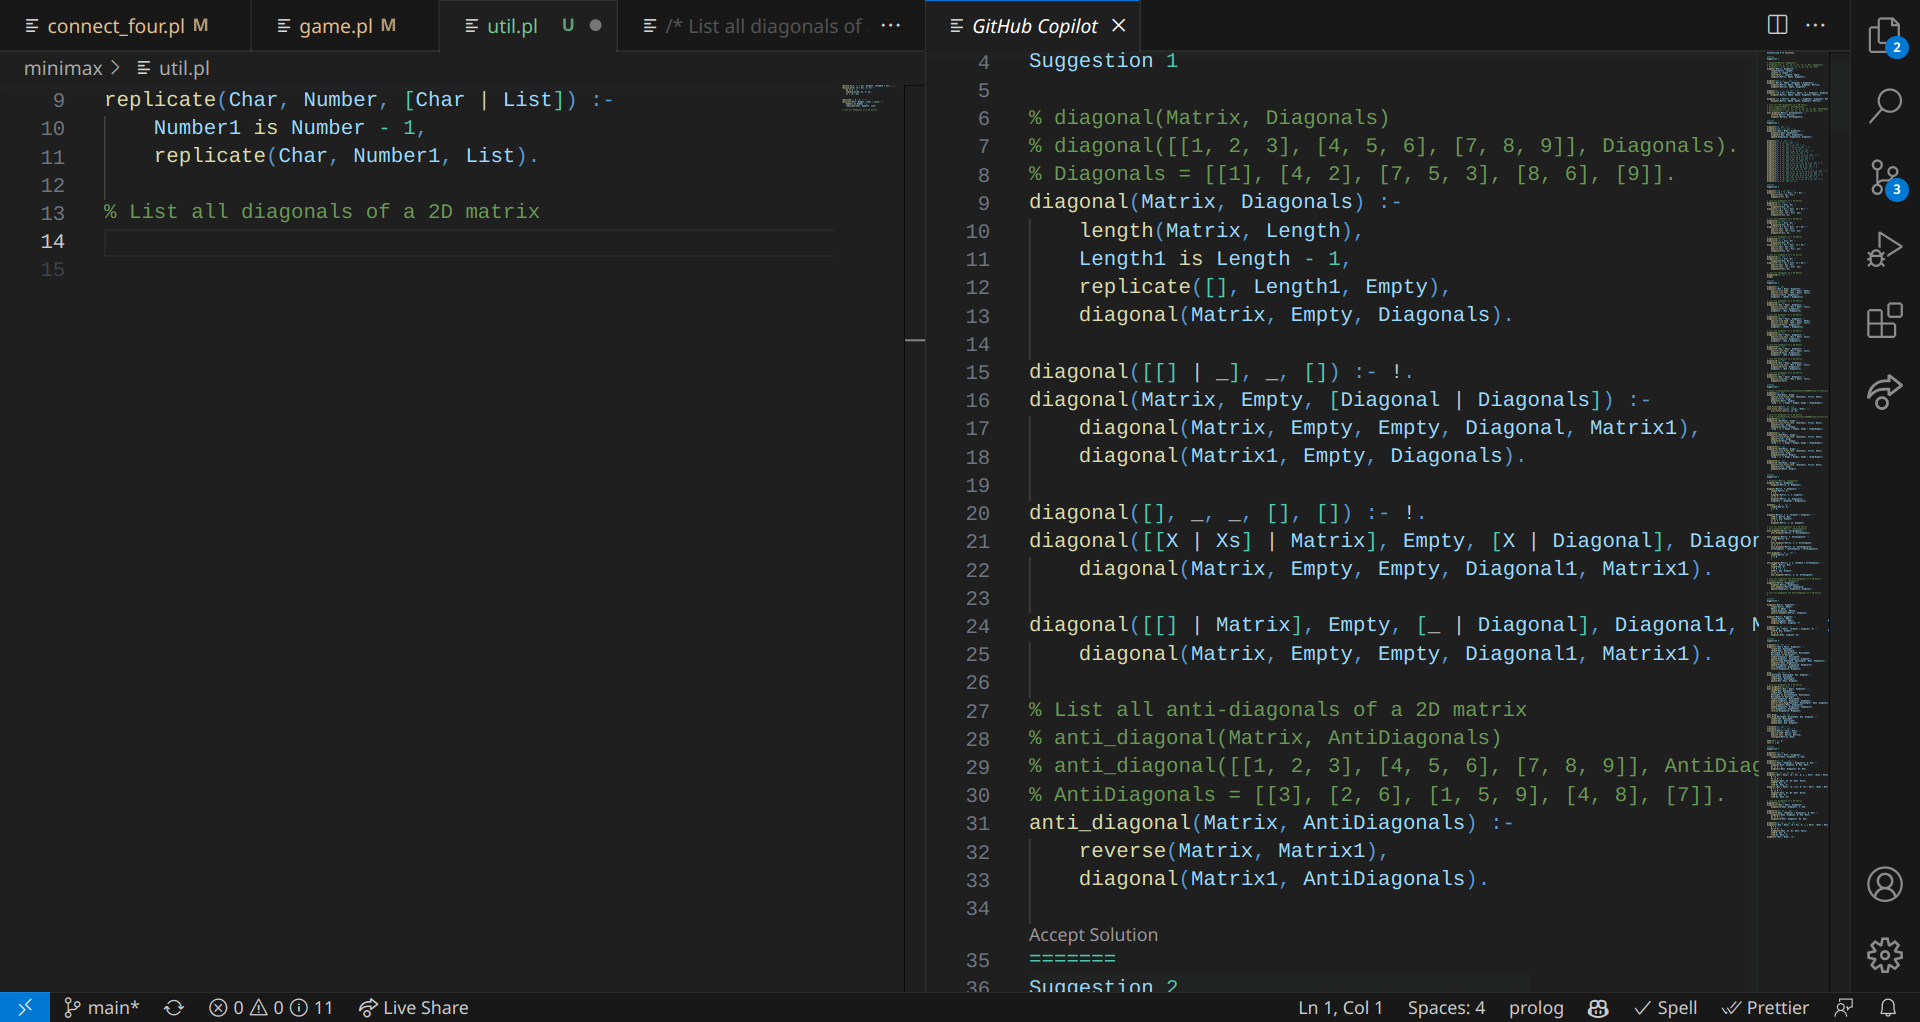
\includegraphics[width=\textwidth]{copilot-not-helpful-diagonal-predicate}
    \caption{GitHub co-pilot suggesting incorrect code to get the diagonals of a 2D matrix}
    \label{fig:copilot_diagonal}
\end{figure}

\end{document}
